\contribution{Bus}
\shortcontributor{CS6230 : CAD for VLSI Project Report}
\shortcontribution{Documentation}
\headnum{13}
\begin{paper}
\renewcommand*{\pagemark}{}

\section*{Packages\sdot}
\texttt{import Bus :: * ;}
\section*{Description\sdot}
The Bus library includes interface, transactor, and function definition to fulfill a minimal Bus with Bluespec System Verilog. The implementation of BusMasters and Slaves can be attached to other devices employing naive Get and Put connections.

\begin{figure}[H]
\centering
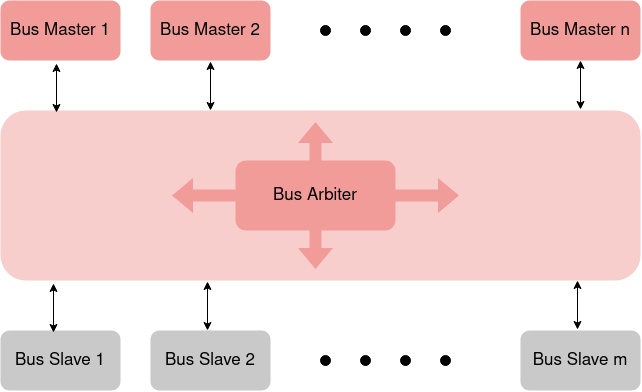
\includegraphics[width=8cm]{Images/Overview-Bus.png}
\caption{\content The bus system.}
\end{figure}\\


\section*{Data Structures\sdot}
Within the Bus, the data is composed of the following data structures: the \texttt{ControlSignal} contains information about the type of the signal, i.e, \texttt{Read, Write \& Response}. The \texttt{Chunk} datatype contains the entire signal.

\subsection*{Chunk\sdot}
The Chunk is a structure containing all the information to be transacted.

\begin{center}
\begin{longtable}{lll}
\multicolumn{3}{c}{\heavy Chunk\sdot}                                                      \\
\heavy Member  & \heavy Datatype                         & \heavy Valid Values        \\
control & ControlSignal                                  & Read/Write/Response \\
data    & Bit \#(datasize)                               & ..                  \\
addr    & Bit \#(addrsize)                               & ..                  \\
present & Bit \#(PresentSize \# (datasize, granularity)) & ..                 
\end{longtable}
\end{center}

\begin{minted}[
bgcolor=Gray !5
]{Haskell}
typedef enum {Response, Read, Write} ControlSignal deriving (Bits, Eq, FShow);

typedef TLog #(TAdd #(TDiv #(datasize, granularity), 1)) 
PresentSize #(numeric type datasize,
              numeric type granularity);

typedef struct {ControlSignal control;
                Bit #(datasize) data;
                Bit #(addrsize) addr;
                Bit #(PresentSize #(datasize, granularity)) present;}

                Chunk #(numeric type datasize,
                        numeric type addrsize,
                        numeric type granularity) deriving (Bits, FShow);

\end{minted}\\\\

\section*{Bus Interfaces\sdot}
The package includes two major bus interfaces \texttt{BusMaster} and \texttt{BusSlave}. The interface for the bus fabric is \texttt{Bus}. 

\subsection*{BusMaster\sdot}
The BusMaster interface issues \texttt{Read/Write} requests and recieves \texttt{Responses}. The bus master connects with the master device through simple \texttt{Get/Put} interfaces.

\begin{minted}[
bgcolor=Gray !5
]{Haskell}
// An interface for the bus master
// Param datasize   : The width of the databus
// Param addrsize   : The width of the addressbus
// Param granularity: Size of the smallest addressable unit
interface BusMaster #(numeric type datasize,
                      numeric type addrsize, 
                      numeric type granularity);
    // Frontend
    interface Put #(Chunk #(datasize, addrsize, granularity)) job_send;
    interface Get #(Chunk #(datasize, addrsize, granularity)) job_done;

    // Backend
    method Bool valid;
    method Action granted (Bool permission);
    method Action available (Bool availability);
    interface Put #(Chunk #(datasize, addrsize, granularity)) put_states;
    interface Get #(Chunk #(datasize, addrsize, granularity)) get_states;
endinterface

\end{minted}\\\\

\subsection*{BusSlave\sdot}
The BusSlave gets \texttt{Read/Write} requests and issues \texttt{Responses}.

\begin{minted}[
bgcolor=Gray !5
]{Haskell}
// An interface for the bus slave
interface BusSlave #(numeric type datasize,
                     numeric type addrsize, 
                     numeric type granularity);
    // Front end
    interface Get #(Chunk #(datasize, addrsize, granularity)) job_recieve;
    interface Put #(Chunk #(datasize, addrsize, granularity)) job_done;

    // Backend
    method Bool is_address_valid (Bit #(addrsize) addr);
    interface Put #(Chunk #(datasize, addrsize, granularity)) put_states;
    interface Get #(Chunk #(datasize, addrsize, granularity)) get_states;
endinterface

\end{minted}\\\\

\subsection*{Bus\sdot}
The Bus is the medium of communication. It contains the \texttt{Arbiter} which mediates the transactions.


\begin{minted}[
bgcolor=Gray !5,
breaklines
]{Haskell}
// An interface for the bus fabric
interface Bus #(numeric type masters,
                numeric type slaves, 
                numeric type datasize, 
                numeric type addrsize, 
                numeric type granularity);
    interface Put #(Chunk #(datasize, addrsize, granularity)) write_to_bus;
    interface Put #(Chunk #(datasize, addrsize, granularity)) write_to_bus_slave;
    interface Get #(Chunk #(datasize, addrsize, granularity)) read_from_bus;
endinterface
\end{minted}\\\\
\nointend The \texttt{Bus} is connectable with \texttt{BusMaster} & \texttt{BusSlave}. The bus is also connectable with vectors of \texttt{BusMaster} and \texttt{BusSlave}.

\section*{Modules\sdot}
The following constructors are used to create the bus.
\subsubsection*{mkBusSlave\sdot}
Creates the BusSlave interface.
\begin{minted}[
bgcolor=Gray !5,
breaklines
]{Haskell}
// Module defintion for a BusSlave
// Param lower_bound : Lower bound of the Slave address
// Param upper_bound : Upper bound of the Slave address
// Param id          : Integer id for the slave
module mkBusSlave #(Bit #(addrsize) lower_bound,
                    Bit #(addrsize) upper_bound,
                    Integer id) (BusSlave #(datasize, addrsize, granularity));
\end{minted}
\subsection*{mkBusMaster\sdot}
Creates the BusMaster interface.
\begin{minted}[
bgcolor=Gray !5,
breaklines
]{Haskell}
// Module defintion for a BusMaster
// Param id          : Integer id for the master
module mkBusMaster #(Integer id) 
                    (BusMaster #(datasize, addrsize, granularity));
\end{minted}
\subsection*{mkBus\sdot}
Creates the Bus interface.
\begin{minted}[
bgcolor=Gray !5,
breaklines
]{Haskell}
// Module defintion for a Bus fabric
// Param master_vec : A vector of BusMasters
// Param slave_vec  : A vector of BusSlaves
module mkBus #(Vector #(masters, BusMaster #(datasize, addrsize, granularity)) 
                        master_vec,
               Vector #(slaves, BusSlave #(datasize, addrsize, granularity)) 
                        slave_vec) 
              (Bus #(masters, slaves, datasize, addrsize, granularity));
\end{minted}
\end{paper}


